% ****** Start of file apssamp.tex ******
%
%   This file is part of the APS files in the REVTeX 4 distribution.
%   Version 4.0 of REVTeX, August 2001
%
%   Copyright (c) 2001 The American Physical Society.
%
%   See the REVTeX 4 README file for restrictions and more information.
%
% TeX'ing this file requires that you have AMS-LaTeX 2.0 installed
% as well as the rest of the prerequisites for REVTeX 4.0
%
% See the REVTeX 4 README file
% It also requires running BibTeX. The commands are as follows:
%
%  1)  latex apssamp.tex
%  2)  bibtex apssamp
%  3)  latex apssamp.tex
%  4)  latex apssamp.tex
%
\documentclass[prb,aps,twocolumn,preprintnumbers,amsmath,amssymb]{revtex4}
%\documentclass[preprint,showpacs,preprintnumbers,amsmath,amssymb]{revtex4}

% Some other (several out of many) possibilities
%\documentclass[preprint,aps]{revtex4}
%\documentclass[preprint,aps,draft]{revtex4}
%\documentclass[prb,twocolumn,showpacs,preprintnumbers,amsmath,amssymb]{revtex4}% Physical Review B

\usepackage{graphicx}% Include figure files
\usepackage{dcolumn}% Align table columns on decimal point
\usepackage{bm}% bold math
\usepackage[utf8]{inputenc}
\usepackage{url}
%\nofiles

\begin{document}

\title{Espectros atómicos}% Force line breaks with \\

\author{Alejandro Hernández A.}%
 \email{a.hernandez105@uniandes.edu.co}
\author{Daniel Sánchez M.}%
 \email{d.sanches462@uniandes.edu.co}
\affiliation{%
Departamento de Física\\ Universidad de los Andes, Bogotá, Colombia.\\
}%


\date{13 de agosto de 2015}% It is always \today, today,
             %  but any date may be explicitly specified

\begin{abstract}
Este informe presenta los datos obtenidos al medir con un espectrómetro de prima sencillo las líneas espectrales de los siguientes gases: hidrógeno, helio, mercurio, kryptón y argón. Conociendo  la separación entre estas líneas y aplicando el modelo de Bohr, se obtuvo un valor experimental para la constante de Rydberg, a saber, $R_{exp} = (10967597.395 \pm 262058.04)\ m^{-1}$ con un error porcentual de $E\% = 0.055\%$.
\\

%\smallskip
\noindent \textbf{Conceptos clave:} Espectrómetro, modelo de Bohr, líneas espectrales, constante de Rydberg.
\end{abstract}
                             
\maketitle

\section{\label{sec:level1}Introducción.}

Una línea espectral es una línea brillante que resalta en un espectro uniforme y continuo, que resulta de la emisión o absorción de luz en un rango de frecuencias determinado. Este tipo de líneas son típicamente usadas para identificar átomos y moléculas a partir de sus líneas espectrales características.\\

El modelo más sencillo que explica teóricamente la aparición de las líneas espectrales en el espectro atómico es el modelo de Bohr \cite{eisberg}. Partiendo de la relación de de Broglie $\lambda = \frac{h}{mv}$ y de la cuantización del momento angular $L = n\frac{h}{2\pi} = n\hbar, \ n \in \mathbb{N}$, el modelo de Bohr predice que las enerías de los diversos niveles electrónicos del átomo de hidrógeno están dadas por

\begin{equation}
E_{n} = -\frac{Z^2 k^2 e^4 m_{e}}{2 \hbar^2 n^2} \approx -\frac{13.6 Z^2}{n^2}\    
\end{equation}

\noindent
donde $n$ caracteriza el nivel de energía en consideración, $Z$ es el número atómico, $k$ es la constante de Coulomb, $e$ es la carga fundamental y $m_{e}$ la masa del electrón.
\\
Ahora bien, para $Z = 1$, la energía de un fotón emitido por un átomo de hidrógeno cuando un electrón salta de un nivel $n_{i}$ a un nivel $n_{f}$ es

\begin{equation}
\Delta E = E_{i} - E_{f} = \frac{k^2 e^4 m_{e}}{2 \hbar ^2} \left(\frac{1}{n_{f}^2}- \frac{1}{n_{i}^2} \right)  
\end{equation}

Finalmente, al tener en cuenta que la energía de un fotón es $\Delta E = \frac{hc}{\lambda}$, la longitud de onda para un fotón emitido en el salto $n_{i} \rightarrow n_{f}$ es

\begin{equation}
\label{balmer}
\frac{1}{\lambda} = \frac{k^2 e^4 m_{e}}{4 \pi \hbar ^3 c} \left(\frac{1}{n_{f}^2}- \frac{1}{n_{i}^2} \right)  
\end{equation}

La anterior ecuación se conoce como la fórmula de Rydberg y 
\\

\begin{equation}
\label{rydberg}
R = \frac{k^2 e^4 m_{e}}{4 \pi \hbar ^3 c}
\end{equation}

se denomina constante de Rydberg.\\

La denominada serie de Balmer para el hidrógeno se obtiene de \eqref{balmer} fijando $n_{i} = 2$ y $n_{f} = 3,4,5 \dots$.
\section{Montaje experimental}

Con el fin de medir las líneas espectrales de los diversos gases proporcionados, se usó un espectrómetro de prisma sencillo.\\ 

El montaje experimental y el nombre de cada elemento usado durante el laboratorio se muestra a continuación.\\

\begin{figure}[h!]
	\centering
	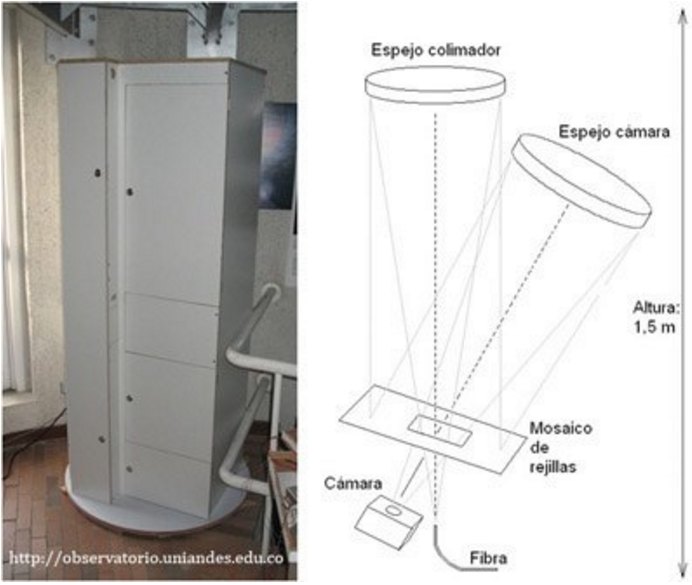
\includegraphics[width=0.5\textwidth]{espectrometro}
	\caption{Componentes de un espectrómetro de prima sencillo.}
\end{figure}

Los pasos seguidos durante el desarrollo del mencionado laboratorio fueron los siguientes:
\\

\begin{enumerate}
	\item \textbf{Enfoque del espectrómetro:} Antes de poner el prisma en el centro del espectrómetro y de realizar las mediciones propiamente dichas se ajustó la altura del espectrómetro para una visualización cómoda, así como los focos del colimador y del telescopio, con el fin de tener una visión lo más clara posible de las líneas espectrales.
	
	\item \textbf{Calibración del espectrómetro:} Tomando como punto de partida el tubo espectral que contenía al helio, se ubicó el prisma sobre la base giratoria y se midieron, con ayuda de una reglilla proyectada, las posiciones de las líneas del espectro de este gas. Finalmente, mediante una curva de la longitud de onda asociada a cada línea de acuerdo a su color vs la posición medida de la línea, se obtuvo una curva de calibración para el espectrómetro.
	
	\item \textbf{Obtención de la constante de Rydberg:} Tras cambiar el tuvo espectral de helio por el de hidrógeno  y usando los resultados de la curva de calibración y el modelo de Bohr, se determinó un valor experimental para la constante de Rydberg, cuyo valor teórico esta dado por \eqref{rydberg}.
	
	\item \textbf{Mediciones para lso demás gases:} Repitiendo el proceso de los dos pasos anteriores y cambiando el tuvo espectral observado, se midieron las líneas espectrales de los demás gases.
\end{enumerate}

\section{Resultados y análisis}

Los resultados de las mediciones de las múltiples líneas espectrales de los diversos gases se muestran en las siguientes tablas.\\

En lo que respecta a la calibración del espectrómetro con helio, los datos fueron los siguientes:

\begin{table}[h!]
	\caption{\label{Tabla 1}Espectro observado para el helio.}
	\begin{ruledtabular}
		\begin{tabular}{ccc}
			Color&$\lambda$ (nm)&Posición(adimensional)\\
			\hline
			Rojo & 667.615 & 8.4\\
			Amarillo & 587.562& 9.6\\
			Verde & 501.567 & 13.0\\
			Azul & 471.314 & 13.2\\
			Azul & 447.148 & 14.5\\
			Morado & 438.793 & 16.0\\
		\end{tabular}
	\end{ruledtabular}
\end{table}

\indent
Donde las longitudes de onda $\lambda$ de cada una de las líneas fueron obtenidas mediante su color \footnote{Espectros obtenidos de la página del NIST (National Institute of Standards and Technology)}. Al graficar  estos datos contra la posición medida de las mismas, en la FIG. \ref{fig:regresion} se observa una aparente relación lineal entre la longitud de onda y la posición medida de la línea, razón por la cual se hizo una regresión lineal sobre los datos. 
\\

El resultado de la regresión fue el siguiente:

\begin{equation}
\label{regresion}
\lambda = (-30.228\ nm)x + (895.376\ nm)
\end{equation}
\noindent
donde x es la posición medida de la línea. El error estándar $s = 3.821$ y correlación $r^2 = 0.939$ justifican la relación lineal propuesta entre los datos. Dado lo anterior, la curva de calibración queda determinada por \eqref{regresion}
\begin{figure}[h!]
	\centering
	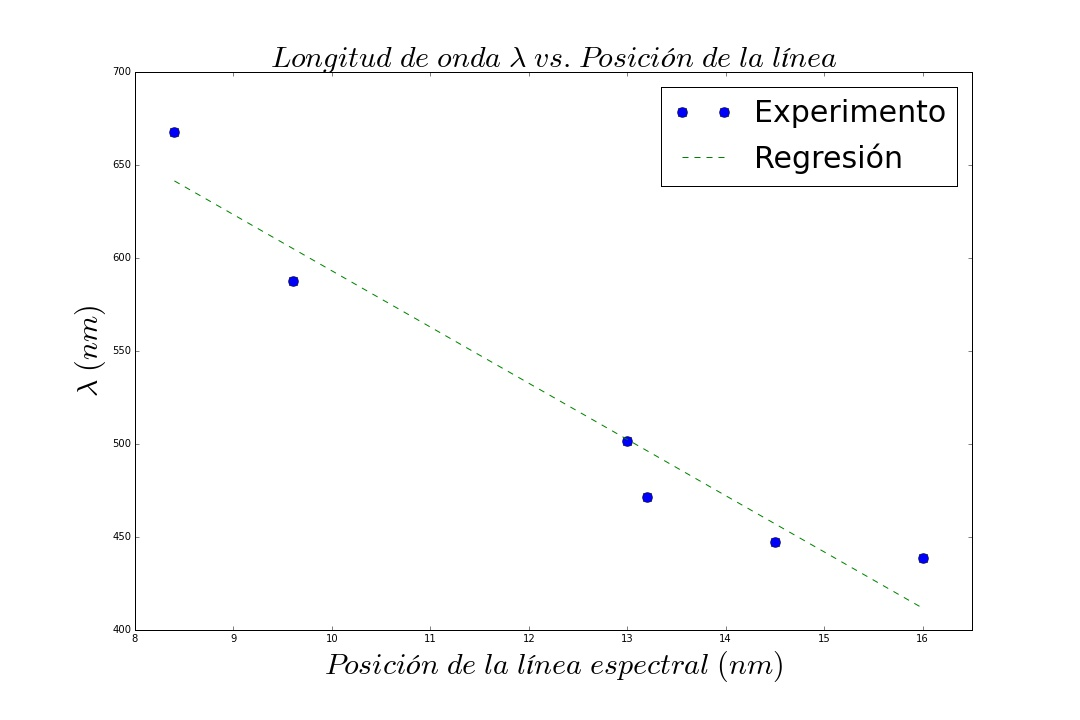
\includegraphics[width=0.5\textwidth]{regresion}
	\caption{Datos expermimentales para el helio.\label{fig:regresion}}
\end{figure}

Ahora bien, con el fin de determinar el valor experimental de la constante de Rydberg es necesario conocer los niveles $n$ entre los cuales se realiza el salto y para esto usamos la serie de Balmer dada por \eqref{balmer}. En este modelo, el nivel\\

Para el caso particular de las líneas observadas para el hidrógeno, los niveles son 

\begin{table}[h!]
\caption{\label{Tabla 6}Niveles usados para el hidrógeno.}
\begin{ruledtabular}
\begin{tabular}{cc}
Color&$n_{i}$\\
\hline
Rojo &3\\
Verde &4\\
Morado &5\\
\end{tabular}
\end{ruledtabular}
\end{table}

Y al hacer nuevamente una regresión con base en \eqref{balmer} se obtiene lo siguiente

\begin{equation}
\frac{1}{\lambda} = (10967597.395\ m^{-1})x + (32266.600\ m^{-1})
\end{equation}

\noindent
con error estándar $s = 262058.04$ y parámetro de correlación $r^2 = 0.999$. Con lo anterior, el valor obtenido para la constante de Rydberg fue

\begin{equation}
R_{exp} = (10967597.395 \pm 262058.049)\ m^{-1}
\end{equation}

Teniendo en cuenta que el valor teórico \footnote{Valor obtenido de https://en.wikipedia.org/wiki/Rydberg\_Constant}  de esta constante es $R_{teo}  = 10973731.685\ m^{-1}$ , el error porcentual de la medida es $E\% = 0.055\%$, motivo por el cual podemos afirmar que las medidas experimentales fueron llevadas a cabo de una buena manera.\\

Para los demás gases, los datos medidos se muestran a continuación.

\begin{table}[h!]
\caption{\label{Tabla 2}Espectro observado para el hidrógeno.}
\begin{ruledtabular}
\begin{tabular}{ccc}
Color&$\lambda$ (nm)&Posición(adimensional)\\
\hline
Rojo & 656.112 & 8.4\\
Verde & 486.008 & 13.7\\
Morado & 433.936 & 15.5\\
\end{tabular}
\end{ruledtabular}
\end{table}

\begin{figure}[h!]
	\centering
	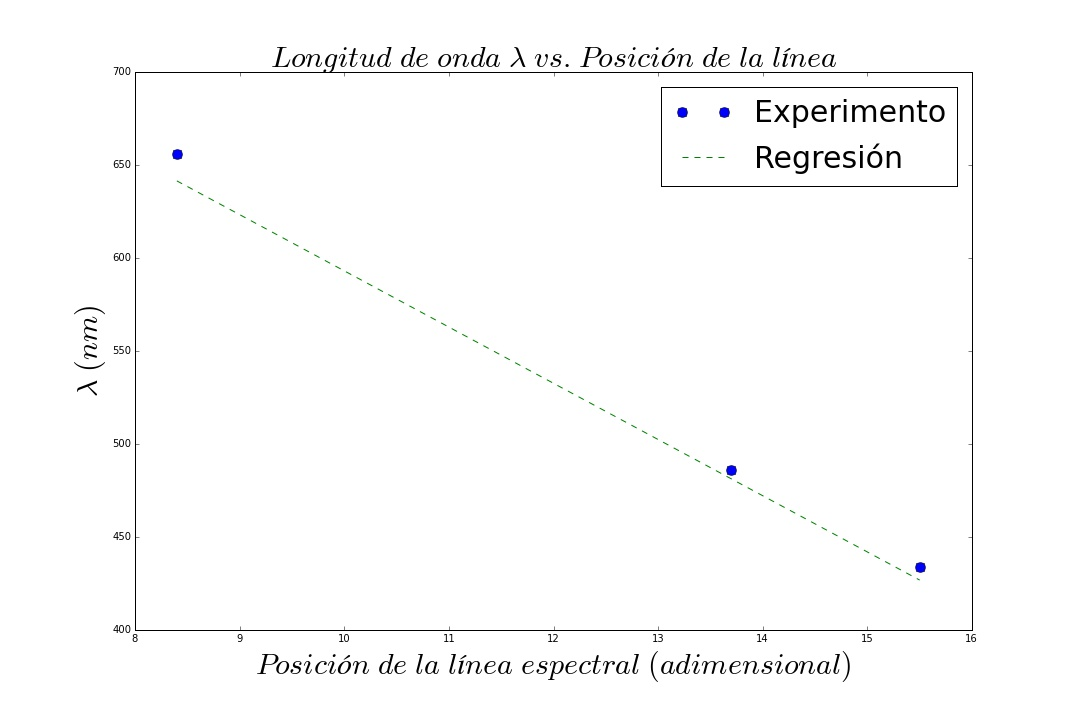
\includegraphics[width=0.5\textwidth]{regresion_hidrogeno}
	\caption{Datos expermimentales para el hidrógeno.}
\end{figure}

\begin{table}[h!]
\caption{\label{Tabla 3}Espectro observado para el mercurio.}
\begin{ruledtabular}
\begin{tabular}{ccc}
Color&$\lambda$ (nm)&Posición(adimensional)\\
\hline
Amarillo & 579.065 & 10.2\\
Verde & 546.074 & 11.3\\
Morado & 435.835 & 16.9\\
\end{tabular}
\end{ruledtabular}
\end{table}

\begin{figure}[h!]
	\centering
	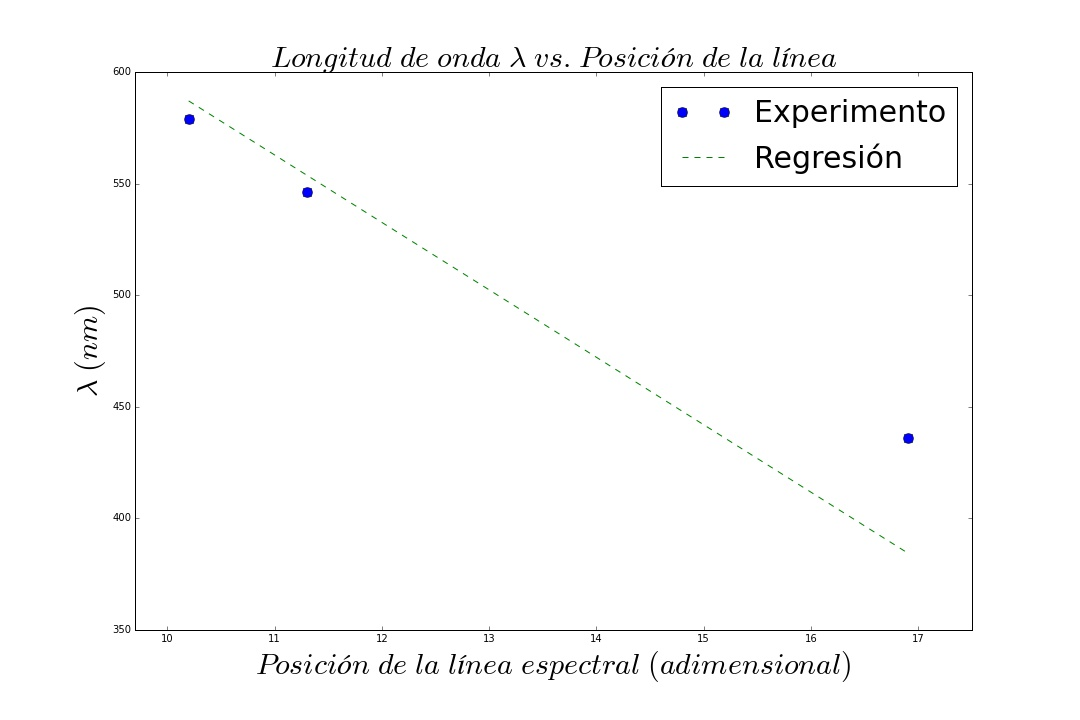
\includegraphics[width=0.5\textwidth,height=0.2\textheight]{regresion_mercurio}
	\caption{Datos expermimentales para el mercurio.}
\end{figure}

\begin{table}[h!]
\caption{\label{Tabla 4}Espectro observado para el argón.}
\begin{ruledtabular}
\begin{tabular}{ccc}
Color&$\lambda$ (nm)&Posición(adimensional)\\
\hline
Rojo & 750.386 & 6.8\\
Naranja & 696.543 & 8.0\\
Verde & 617.227 & 9.5\\
Azul & 487.986 & 12.5\\
Morado & 427.752 & 16.0\\
\end{tabular}
\end{ruledtabular}
\end{table}

\begin{figure}[h!]
	\centering
	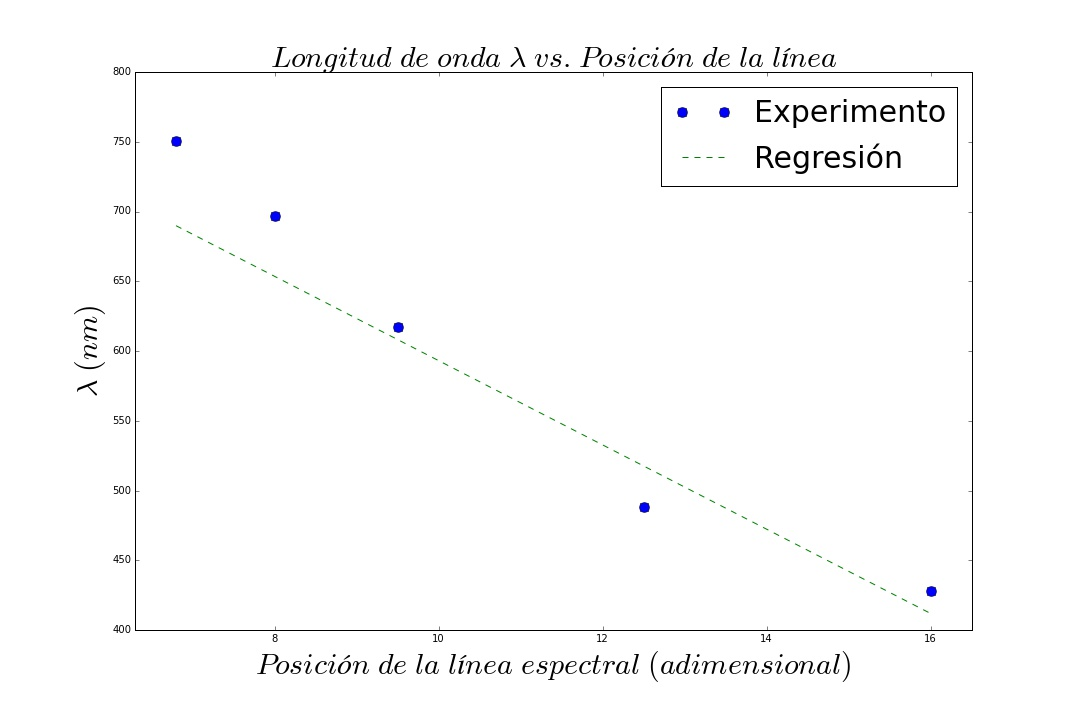
\includegraphics[width=0.5\textwidth]{regresion_argon}
	\caption{Datos expermimentales para el argón.}
\end{figure}

\begin{table}[h!]
\caption{\label{Tabla 5}Espectro observado para el kriptón.}
\begin{ruledtabular}
\begin{tabular}{ccc}
Color&$\lambda$ (nm)&Posición(adimensional)\\
\hline
Rojo & 728.978 & 6.9\\
Naranja & 642.018 & 8.3\\
Verde & 587.091 & 10.5\\
Azul & 533.341 & 12.0\\
Morado & 435.547 & 14.9\\
\end{tabular}
\end{ruledtabular}
\end{table}

\begin{figure}[h!]
	\centering
	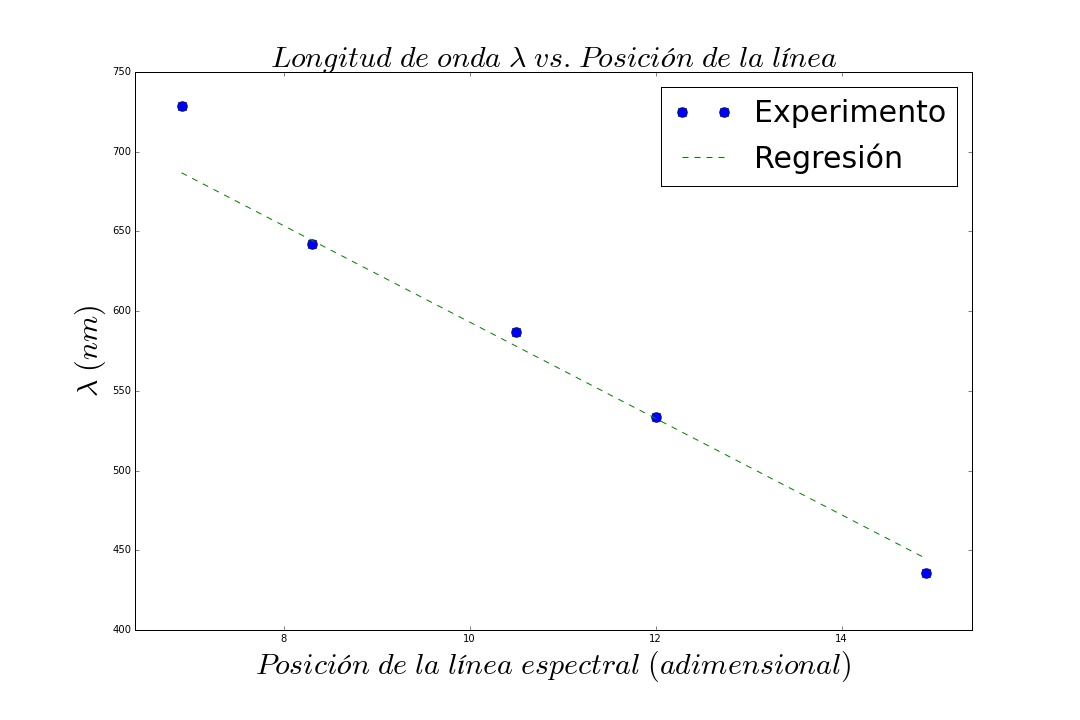
\includegraphics[width=0.5\textwidth]{regresion_kripton}
	\caption{Datos expermimentales para el kriptón.}
\end{figure}

Cabe aclarar que en las gráficas anteriores, la línea correspondiente a la regresión hace alusión a la curva de calibración hecha para el helio. Teniendo en cuenta lo anterior, podemos afirmar que los datos medidos se ajustan bien a la mencionada curva de calibración.

\section{Conclusiones}

\begin{itemize}

	\item La curva de calibración obtenida para el helio, se ajusta bien a las líneas espectrales obervadas para los demás gases, tal y como se muestra en las gráficas de la sección anterior.
	
	\item El valor experimental obtenido para la constante de Rydberg $R_{exp} = (10967597.395 \pm 262058.049)\ m^{-1}$ es muy exacto dado a que el error porcentual de la medida fue de $E\% = 0.055\%$.
		
	\item La observación realizada de las líneas espectrales perimten concluir la validez del modelo de Bohr (o la serie de Balmer) para explicar el espectro de emisión de átomos con un solo electrón, y al tener la hipótesis de cuantización del momento angular, los resultados experimentales obtenidos permiten constatar unad las primeras ideas acerca de cuantización en física.
	
	\item Si bien se obtuvieron buenos resultados, es importante resaltar que tanto la intensidad de las líneas espectrales de los diversos gases, como el grosor de las mismas, da pie para pensar acerca de la realización de medidas con instrumentos de mayor resolución con el fin de obtener mediciones más exactas de la posición de las mismas.
	
\end{itemize}

\begin{thebibliography}{99}
\bibitem{eisberg} R. Eisberg, {\it Quantum Physics of Atoms, Molecules, Solids, Nuclei and Particles}{John Wiley \& Sons, USA, 1985}.\\
\end{thebibliography}

\end{document}
%
% ****** End of file apssamp.tex ******
